\documentclass[12pt, twoside]{book}
%\documentclass[12pt, oneside]{book}  % jednostranna tlac

%spravne nastavenie okrajov
\usepackage[a4paper,top=2.5cm,bottom=2.5cm,left=3.5cm,right=2cm]{geometry}
%zapnutie fontov pre UTF8 kodovanie
\usepackage[utf8]{inputenc}
\usepackage[T1]{fontenc}

%zapnutie slovenskeho delenia slov
%a automatickych nadpisov ako Obsah, Obrázok a pod. v slovencine
\usepackage[slovak]{babel} % vypnite pre prace v anglictine!

%nastavenie riadkovania podla smernice
\linespread{1.25} % hodnota 1.25 by mala zodpovedat 1.5 riadkovaniu

% balicek na vkladanie zdrojoveho kodu
\usepackage{listings}

% nastavenia balicka listings
\renewcommand{\lstlistingname}{Algoritmus}
\lstset{extendedchars=true, basicstyle=\small, frame=lines,
    commentstyle=\color{olive}\textit, keywordstyle=[1]\color{blue},
    literate=
    {á}{{\'a}}1 {ä}{{\"a}}1 {č}{{\v{c}}}1 {ď}{{\v{d}}}1 {é}{{\'e}}1 {í}{{\'i}}1
    {ĺ}{{\'l}}1 {ľ}{{\v{l}}}1 {ň}{{\v{n}}}1 {ó}{{\'o}}1 {ô}{{\^o}}1 {š}{{\v{s}}}1
    {ť}{{\v{t}}}1 {ú}{{\'u}}1 {ý}{{\'y}}1 {ž}{{\v{z}}}1
    {Á}{{\'A}}1 {Č}{{\v{C}}}1 {Ď}{{\v{D}}}1 {É}{{\'E}}1 {Í}{{\'I}}1 {Ĺ}{{\'L}}1 
    {Ľ}{{\v{L}}}1 {Ň}{{\v{N}}}1 {Ó}{{\'O}}1 {Š}{{\v{S}}}1 {Ť}{{\v{T}}}1 {Ú}{{\'U}}1
    {Ý}{{\'Y}}1 {Ž}{{\v{Z}}}1
}
\lstdefinelanguage{AVR}{
    keywords={clr, eor, cpi, breq, inc, tst, brne, ldi, sbi, cbi, nop, add, sub, mov, or, dec, ldr, str},
    sensitive=false,
    comment=[l]{;},
}

% balicek na vkladanie obrazkov
\usepackage{graphicx}
\usepackage{subfig}
% balicek na vkladanie celych pdf dokumentov
\usepackage{pdfpages}
% balicek na vkladanie diagramov
\usepackage{pgfplots}
\pgfplotsset{width=0.6\textwidth,compat=1.9}
% balicek na spravne formatovanie URL
\usepackage{url}
% balicek na hyperlinky v ramci dokumentu
% zrusime farebne ramiky okolo liniek
\usepackage[hidelinks,breaklinks]{hyperref}



% -------------------
% --- Definicia zakladnych pojmov
% --- Vyplnte podla vasho zadania, rok ma byt rok odovzdania
% -------------------
\def\mfrok{2023}
\def\mfnazov{Útoky na hardvér\\pomocou indukovania chýb}
\def\mftyp{Bakalárska práca}
\def\mfautor{Dennis Vita}
\def\mfskolitel{RNDr. Richard Ostertág, PhD. }

\def\mfmiesto{Bratislava, \mfrok}

\def\mfodbor{ Informatika}
\def\program{ Informatika }
\def\mfpracovisko{ FMFI.KI - Katedra informatiky }

\begin{document}
\frontmatter
\pagestyle{empty}

% -------------------
% --- Obalka ------
% -------------------
\begin{center}
\sc\large
Univerzita Komenského v Bratislave\\
Fakulta matematiky, fyziky a informatiky

\vfill

{\LARGE\mfnazov}\\
\mftyp
\end{center}

\vfill

{\sc\large 
\noindent \mfrok\\
\mfautor
}

\cleardoublepage
% --- koniec obalky ----


% -------------------
% --- Titulný list
% -------------------
\noindent
\setcounter{page}{1}

\begin{center}
\sc  
\large
Univerzita Komenského v Bratislave\\
Fakulta matematiky, fyziky a informatiky

\vfill

{\LARGE\mfnazov}\\
\mftyp
\end{center}

\vfill

\noindent
\begin{tabular}{ll}
Študijný program: & \program \\
Študijný odbor: & \mfodbor \\
Školiace pracovisko: & \mfpracovisko \\
Školiteľ: & \mfskolitel \\
\end{tabular}

\vfill


\noindent \mfmiesto\\
\mfautor

\cleardoublepage
% --- Koniec titulnej strany


% -------------------
% --- Zadanie z AIS
% -------------------
\newpage 
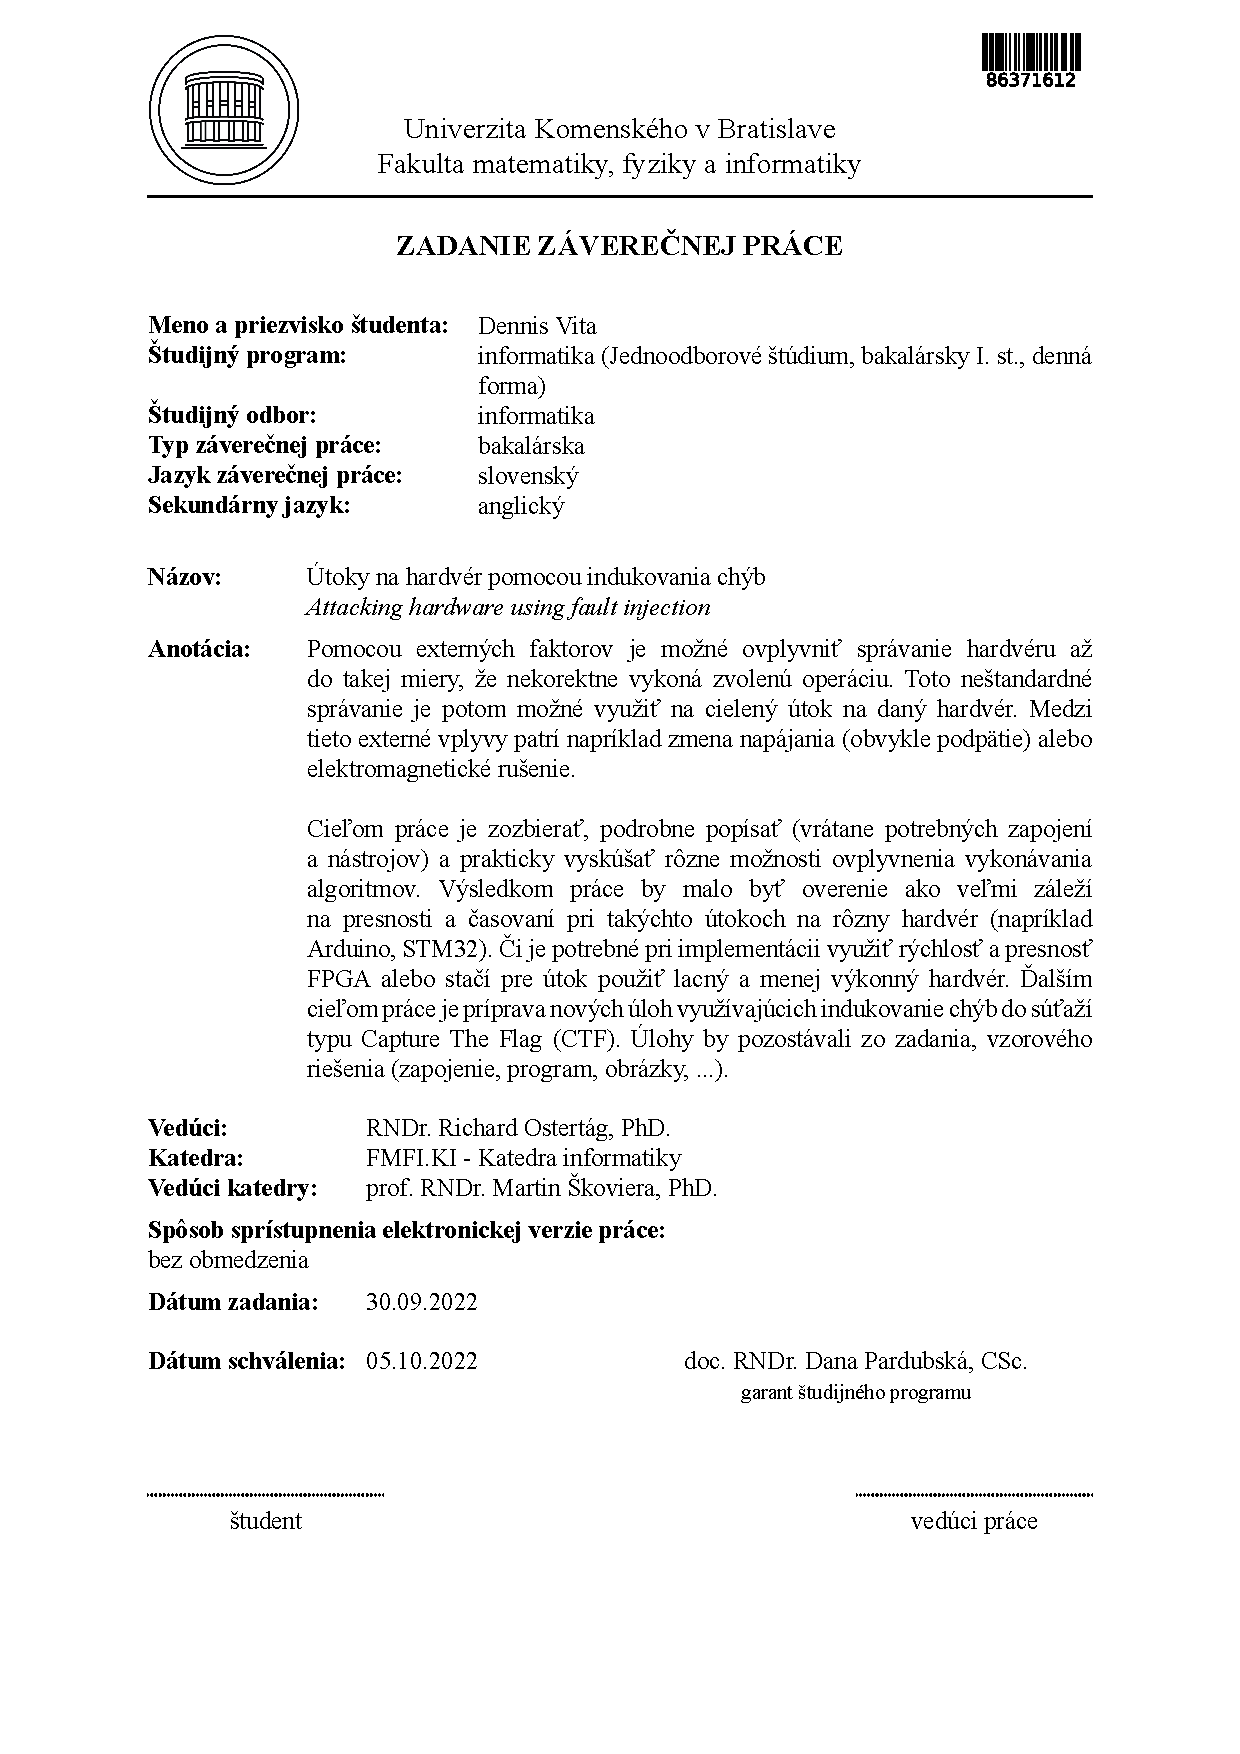
\includepdf{images/zadanie.pdf}

\cleardoublepage
% --- Koniec zadania


% -------------------
%   Poďakovanie - nepovinné
% -------------------
\newpage
\pagestyle{plain}
~

\vfill
{\bf Poďakovanie:} Ďakujem vedúcemu bakalárskej práce RNDr. Richardovi Ostertágovi, PhD. za odborné vedenie, metodickú pomoc, podnetné nápady, pripomienky a~konzultácie pri písaní práce. Ďakujem aj Tomášovi Stykovi za poskytnutie dodatočnej pomoci pri návrhu implementácie niektorých častí práce.\\

Táto práca vznikla aj vďaka podpore v rámci Operačného programu Integrovaná infraštruktúra pre projekt: Advancing University Capacity and Competence in Research, Development and Innovation (ACCORD), spolufinancovaný zo zdrojov Európskeho fondu regionálneho rozvoja.
% --- Koniec poďakovania


% -------------------
%   Abstrakt - Slovensky
% -------------------
\newpage 
\section*{Abstrakt}

Vplyvom externých fyzikálnych faktorov (zmena napájania, elektromagnetické rušenie a pod.) je možné ovplyvniť činnosť hardvéru až do takej miery, že nekorektne vykoná niektorú operáciu. Indukovanie chýb je technika útoku, ktorá zneužíva toto správanie a~možno pomocou nej špecifickým spôsobom zaútočiť na konkrétny hardvér. Pri správnom načasovaní na kritickú časť programu je možné cielene ovplyvniť daný hardvér, napríklad s účelom obísť bezpečnostný mechanizmus alebo narušiť implementáciu kryptografického algoritmu. Jedným cieľom práce je overiť, či aj lacným hardvérom možno realizovať úspešný útok. Zároveň sa v práci zaoberáme podrobnou analýzou vybraných útokov a ich možným dopadom na vybraný hardvér (mikrokontrolér ATMega328P). Cieľom je aj zistiť, aké možnosti indukovania chýb pre útočníka lacný hardvér poskytuje, napríklad vynechanie inštrukcie, ovplyvnenie výsledku operácie a~pod. Výsledky analýzy na záver demonštrujeme úspešnými útokmi na vytvorené cvičné príklady programov.

\paragraph*{Kľúčové slová:} indukovanie chýb, mikrokontrolér, zmena napájania
% --- Koniec Abstrakt - Slovensky


% -------------------
% --- Abstrakt - Anglicky 
% -------------------
\newpage 
\section*{Abstract}

The influence of external physical factors (power supply voltage changes, electromagnetic interference, etc.) can affect the operation of hardware to such an extent that it may incorrectly execute an operation. Fault injection is an attack technique that exploits this behavior and can be used to attack specific hardware. By proper timing and targeting a well-chosen part of a program, it is possible to deliberately influence the targeted hardware, for example, to bypass a security mechanism or cause faults in an implementation of a cryptographic algorithm. One goal of this thesis is to verify whether successful attacks can also be performed using inexpensive hardware. Additionally, the thesis focuses on a detailed analysis of selected attacks and their potential impact on specific hardware (the ATMega328P microcontroller). The aim is also to explore what fault injection capabilities inexpensive hardware to an attacker provides, such as skipping an instruction or influencing the result of an operation.. The analysis results are demonstrated by successful attacks on simple program examples.


\paragraph*{Keywords:} fault injection, microcontroller, power glitch
% --- Koniec Abstrakt - Anglicky


% -------------------
% --- Predhovor - v informatike sa zvacsa nepouziva
% -------------------
%\newpage 
%
%\chapter*{Predhovor}
%
%Predhovor je všeobecná informácia o práci, obsahuje hlavnú charakteristiku práce 
%a okolnosti jej vzniku. Autor zdôvodní výber témy, stručne informuje o cieľoch 
%a význame práce, spomenie domáci a zahraničný kontext, komu je práca určená, 
%použité metódy, stav poznania; autor stručne charakterizuje svoj prístup a svoje 
%hľadisko. 
%
% --- Koniec Predhovor


% -------------------
% --- Obsah
% -------------------
\newpage 

\tableofcontents
% ---  Koniec Obsahu


% -------------------
% --- Zoznamy tabuliek, obrázkov - nepovinne
% -------------------
\newpage 

\listoffigures
\listoftables
% ---  Koniec Zoznamov


\mainmatter
\pagestyle{headings}


\input 00-uvod.tex 

\input 01-teoria.tex

\input 02-hardver.tex

\input 03-utoky.tex

\input 04-CTF.tex

\input 05-zaver.tex


% -------------------
% --- Bibliografia
% -------------------
\newpage	

\backmatter

\thispagestyle{empty}
\clearpage

\bibliographystyle{plain}
\bibliography{literatura} 
%---koniec Referencii


% -------------------
%--- Prilohy---
% -------------------


\input 06-prilohaCD.tex

\end{document}